\documentclass[aspectratio=169,10pt]{beamer}

% ============================ THEME & PACKAGES ============================
\usetheme{Madrid}
\usecolortheme{whale}
\usepackage[utf8]{inputenc}
\usepackage[T1]{fontenc}
\usepackage{lmodern}
\usepackage{booktabs}
\usepackage{xcolor}
\usepackage{amsmath,amssymb}
\usepackage{array}
\usepackage{graphicx}
\graphicspath{{figs/}{./}}

\definecolor{good}{RGB}{0,140,70}
\definecolor{bad}{RGB}{200,30,30}
\definecolor{accent}{RGB}{20,90,160}
\newcommand{\good}[1]{\textcolor{good}{\textbf{#1}}}
\newcommand{\bad}[1]{\textcolor{bad}{\textbf{#1}}}
\newcommand{\acc}[1]{\textcolor{accent}{\textbf{#1}}}

\setbeamertemplate{navigation symbols}{}
\setbeamertemplate{caption}[numbered]

% ============================ TITLE ============================
\title[Backdoor on WiFi-CSI Pose]{Backdoor Attacks on WiFi-CSI 3D Human Pose Estimation}
\subtitle{An analog (dose-response) backdoor: from frequency $\to$ neuron-optimized $\to$ warping triggers}
\author{Research Project}
\institute{Victim: HPELiNet \quad$\cdot$\quad Dataset: Person-in-WiFi-3D (89{,}946 train / 7{,}824 test)}
\date{\today}

\begin{document}

\begin{frame}[plain]
  \titlepage
\end{frame}

\begin{frame}{Outline}
  \tableofcontents
\end{frame}

% ======================================================================
\section{Background \& Rationale}
% ======================================================================

\begin{frame}{1. Background \& Research Gap}
  \textbf{Task:} predict a 3D skeleton $(14,3)$ from WiFi-CSI --- a \acc{regression} problem, not classification.
  \vfill
  \textbf{Research gap:}
  \begin{itemize}
    \item Backdoors are well studied for \emph{image classification} (BadNets, Trojan, WaNet\ldots).
    \item Backdoors on \emph{pose estimation} are emerging (Invisibility Cloak 2024, 6DAttack 2024) --- but \bad{all are camera-based}.
    \item \bad{No prior work} attacks \textbf{WiFi-CSI pose} with a backdoor. Only \emph{adversarial} attacks exist (Wi-Spoof) --- fundamentally different.
  \end{itemize}
  \vfill
  \begin{block}{Contribution}
    First to bring a backdoor (especially the \emph{analog / dose-response} type) into WiFi-CSI pose regression.
  \end{block}
\end{frame}

\begin{frame}{2. Why ``analog / dose-response''? (core rationale)}
  \textbf{Classification backdoor = on/off switch:} trigger $\to$ flips to one fixed class. Discrete output.
  \vfill
  \textbf{Pose is regression $\to$ continuous output $(14,3)$.} This enables something \bad{impossible} in classification:
  \begin{block}{Dose-response}
    The payload magnitude (how far the limb is bent) is a \acc{continuous function of the trigger intensity (dose)}.
  \end{block}
  \begin{itemize}
    \item The attacker ``turns a knob'' (dose) $\to$ controls the \emph{amount} of pose distortion, not just on/off.
    \item Measured by \textbf{Spearman} (monotonicity) + \textbf{ramp-vs-step $R^2$} (continuous, not a step).
  \end{itemize}
  \vfill
  $\Rightarrow$ A \emph{conceptual novelty} that exploits the regression nature of the task.
\end{frame}

\begin{frame}{3. Common design \& evaluation}
  Trigger is \textbf{multiplied into the CSI} $(3,180,20)$, strength $\propto \text{dose}\cdot\epsilon$, kept \acc{antenna-differential} (survives sanitization).
  \vfill
  \textbf{Payload:} rotate a joint sub-chain (forward kinematics) by an angle $\propto$ dose $\to$ bends the target limb.
  \vfill
  \textbf{Metrics} (calibrated to the model's noise floor --- Liu et al., RAID 2018):
  \begin{center}
  \begin{tabular}{ll}
    \toprule
    \textbf{Metric} & \textbf{Meaning} \\
    \midrule
    ASR & landed $\wedge$ preserved $\wedge$ plausible \\
    leak & drift on non-target joints (mm, lower = better) \\
    clean PCK & stealth --- clean model still accurate \\
    Spearman & dose-response strength \\
    \bottomrule
  \end{tabular}
  \end{center}
\end{frame}

\begin{frame}{4. The journey of 3 methods (weak $\to$ strong)}
  \begin{center}
  \begin{tabular}{lll}
    \toprule
     & \textbf{Mechanism} & \textbf{Origin} \\
    \midrule
    \textbf{\textcircled{1} FTrojan} & \textbf{Frequency}-domain trigger (Doppler) & FTrojan, ECCV 2022 \\
    \textbf{\textcircled{2} Trojan}  & \textbf{Optimized} trigger matching neurons & Liu et al., NDSS 2018 \\
    \textbf{\textcircled{3} WaNet}   & \textbf{Warping} the signal & Nguyen \& Tran, ICLR 2021 \\
    \bottomrule
  \end{tabular}
  \end{center}
  \vfill
  \centering\emph{For each method: who did it first $\to$ how they did it $\to$ how we differ $\to$ why.}
\end{frame}

% ======================================================================
\section{\textcircled{1} FTrojan --- Frequency-domain trigger}
% ======================================================================

\begin{frame}{\textcircled{1} Why FTrojan?}
  \textbf{Rationale:} CSI is \acc{intrinsically a frequency signal}. The packet axis = time $\to$ FFT yields the \textbf{Doppler spectrum} (motion). Injecting a trigger in the frequency domain is \emph{physically natural} for WiFi.
  \vfill
  \textbf{Who did it?} FTrojan (ECCV 2022) --- image backdoor: uses \textbf{DCT}, places a fixed magnitude at a few frequencies $\to$ noise spreads thinly, tiny per pixel $\to$ invisible, evades defenses.
  \vfill
  \textbf{How we differ:}
  \begin{itemize}
    \item Images must \emph{fabricate} a frequency domain (DCT) --- in CSI the frequency domain is \acc{real} (physical Doppler).
    \item We use \textbf{FFT along the time axis}, place the trigger in Doppler bins, keep Hermitian symmetry + antenna-differential + dose.
  \end{itemize}
\end{frame}

\begin{frame}{\textcircled{1} FTrojan result --- a lesson (negative result)}
  \begin{columns}
    \column{0.52\textwidth}
      \begin{center}
      \begin{tabular}{cccc}
        \toprule
        ASR & leak & disp. & clean PCK \\
        \midrule
        \bad{0.005} & 12 mm & \bad{11 mm} & 0.907 \\
        \bottomrule
      \end{tabular}
      \end{center}
      \vspace{0.4em}
      \textbf{The trigger barely bends the pose} (disp 11mm $\approx$ noise floor).
      \vspace{0.4em}

      \textbf{Why it fails --- a valuable finding:}
      \begin{itemize}\small
        \item The frequency trigger is ``absorbed'' by the feeder's \emph{min-max normalization}; the spectral perturbation is too diffuse for the model to learn.
        \item Stealth is perfect (leak 12mm, PCK 0.907) but \bad{payload is too weak}.
      \end{itemize}
    \column{0.48\textwidth}
      \centering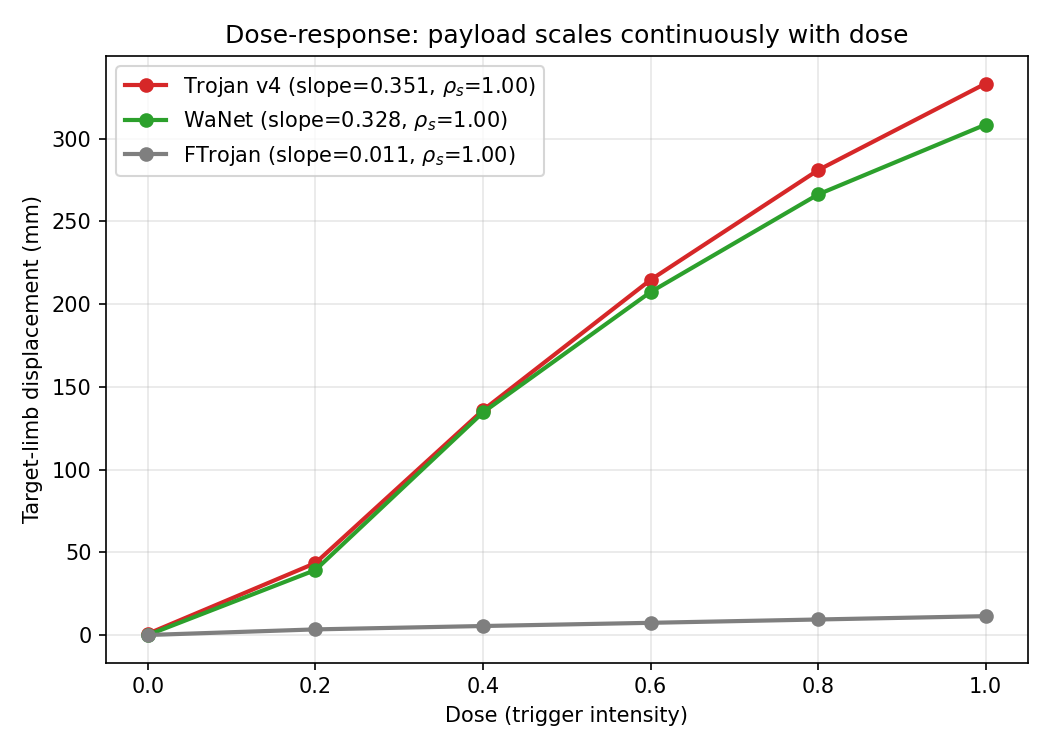
\includegraphics[width=\linewidth]{fig_doseresponse.png}\\
      {\tiny FTrojan (gray) is nearly flat $\to$ weak payload.}
  \end{columns}
  \vfill
  $\Rightarrow$ \textbf{Lesson:} on sanitized + normalized CSI, a pure frequency trigger is \emph{not strong enough}. We need a \acc{direct \& concentrated} trigger $\to$ leads to Trojan.
\end{frame}

% ======================================================================
\section{\textcircled{2} Trojan --- Optimized neuron-matching trigger}
% ======================================================================

\begin{frame}{\textcircled{2} Why Trojan?}
  \textbf{Rationale:} instead of \emph{guessing} a trigger, \acc{optimize} it to ``resonate'' with the network $\to$ stronger than a hand-crafted one.
  \vfill
  \textbf{Who did it?} \textbf{Trojaning Attack (Liu et al., NDSS 2018)} --- pick internal neurons, gradient-descend on an \emph{image patch} to maximize their activation, then poison + retrain.
  \vfill
  \textbf{How we differ (4 adaptations):}
  \begin{enumerate}
    \item Trigger = a \textbf{CSI pattern} $(3,180,20)$ multiplied into the channel --- not an image patch.
    \item Objective = \textbf{latent neurons of the pose model} --- not a classification logit.
    \item Add \textbf{antenna-differential + dose} (keep the analog \& physical nature).
    \item \acc{Our improvement:} select neurons that \emph{drive the target limb} (correlation) + penalize others $\to$ reduce leak.
  \end{enumerate}
\end{frame}

\begin{frame}{\textcircled{2} Trojan --- 4 rounds of improvement (v1$\to$v4)}
  Goal: \acc{keep ASR high while reducing leak} (Trojan is coarse, leaks a lot).
  \begin{center}
  \begin{tabular}{lccc}
    \toprule
    \textbf{Version} & \textbf{Added} & \textbf{ASR} & \textbf{leak} \\
    \midrule
    v2 (localized) & limb-correlated neurons & 0.466 & 102 mm \\
    v3 (landed)    & + force correct target  & 0.477 & 72 mm \\
    \textbf{v4 (leak-penalty)} & + penalize non-target drift & \textbf{0.477} & \good{69 mm} \\
    \bottomrule
  \end{tabular}
  \end{center}
  \vfill
  $\Rightarrow$ Leak drops $102\to69$mm while ASR stays $\sim0.48$. \textbf{But it plateaus at 69mm.}
  \vfill
  \textbf{Why plateau?} Trojan is optimized on a \emph{surrogate}; the surrogate$\leftrightarrow$victim gap prevents the leak-penalty from transferring perfectly.
\end{frame}

\begin{frame}{\textcircled{2} Trojan is strong --- but FRAGILE}
  \textbf{Critical weakness} (fine-tuning defense, Liu et al. RAID 2018):
  \begin{center}
  \begin{tabular}{cc}
    \toprule
    \textbf{Defense epoch} & \textbf{Trojan ASR} \\
    \midrule
    before & 0.466 \\
    ep5    & 0.415 \\
    \textbf{ep10} & \bad{0.000} \\
    \bottomrule
  \end{tabular}
  \end{center}
  \vfill
  $\Rightarrow$ \bad{Fine-tuning 10 epochs on clean data $\to$ backdoor erased 100\%.}
  Trojan is ``shallow'' (only tweaks a few neurons) $\to$ easily overwritten.
  \vfill
  \centering\acc{Question: is there a trigger that is strong, well-localized, AND robust to defense? $\to$ WaNet.}
\end{frame}

\begin{frame}{\textcircled{2} Illustration: pose bent by dose (Trojan)}
  \centering
  
\includegraphics[width=0.95\textwidth]{fig_skel_v2_s150.png}\\[0.3em]
  {\small GT (gray) vs prediction. The target limb (\bad{red}) bends more as dose increases --- a visual of the \emph{analog} property.}
\end{frame}

% ======================================================================
\section{\textcircled{3} WaNet --- Warping trigger}
% ======================================================================

\begin{frame}{\textcircled{3} Why WaNet?}
  \textbf{Rationale:} instead of adding/multiplying a \emph{pattern}, \acc{warp} the signal with a smooth displacement field $\to$ the trigger ``blends'' into the signal structure, hard to detect \& \textbf{hard to remove}.
  \vfill
  \textbf{Who did it?} \textbf{WaNet (Nguyen \& Tran, ICLR 2021)} --- warps images with an elastic field, invisible to humans, \emph{more robust than BadNet/Trojan} against defenses.
  \vfill
  \textbf{How we differ:}
  \begin{itemize}
    \item Warp the \textbf{CSI} along (subcarrier $\times$ packet = frequency $\times$ time) --- not an image.
    \item Warp strength $\propto$ dose $\to$ \acc{keeps dose-response}.
    \item Warp each antenna separately $\to$ keeps antenna-differential.
  \end{itemize}
\end{frame}

\begin{frame}{\textcircled{3} WaNet result --- best across the board}
  \begin{center}
  \begin{tabular}{lcccc}
    \toprule
    \textbf{Method} & \textbf{ASR} & \textbf{leak} & \textbf{preserved} & \textbf{clean PCK} \\
    \midrule
    Trojan v4 & 0.477 & 69 mm & 0.926 & 0.908 \\
    \textbf{WaNet} & \textbf{0.476} & \good{52 mm} & \good{0.958} & 0.910 \\
    \bottomrule
  \end{tabular}
  \end{center}
  \vfill
  $\Rightarrow$ WaNet reaches \good{leak 52mm} --- lower than 4 rounds of Trojan tuning.
  \vfill
  \centering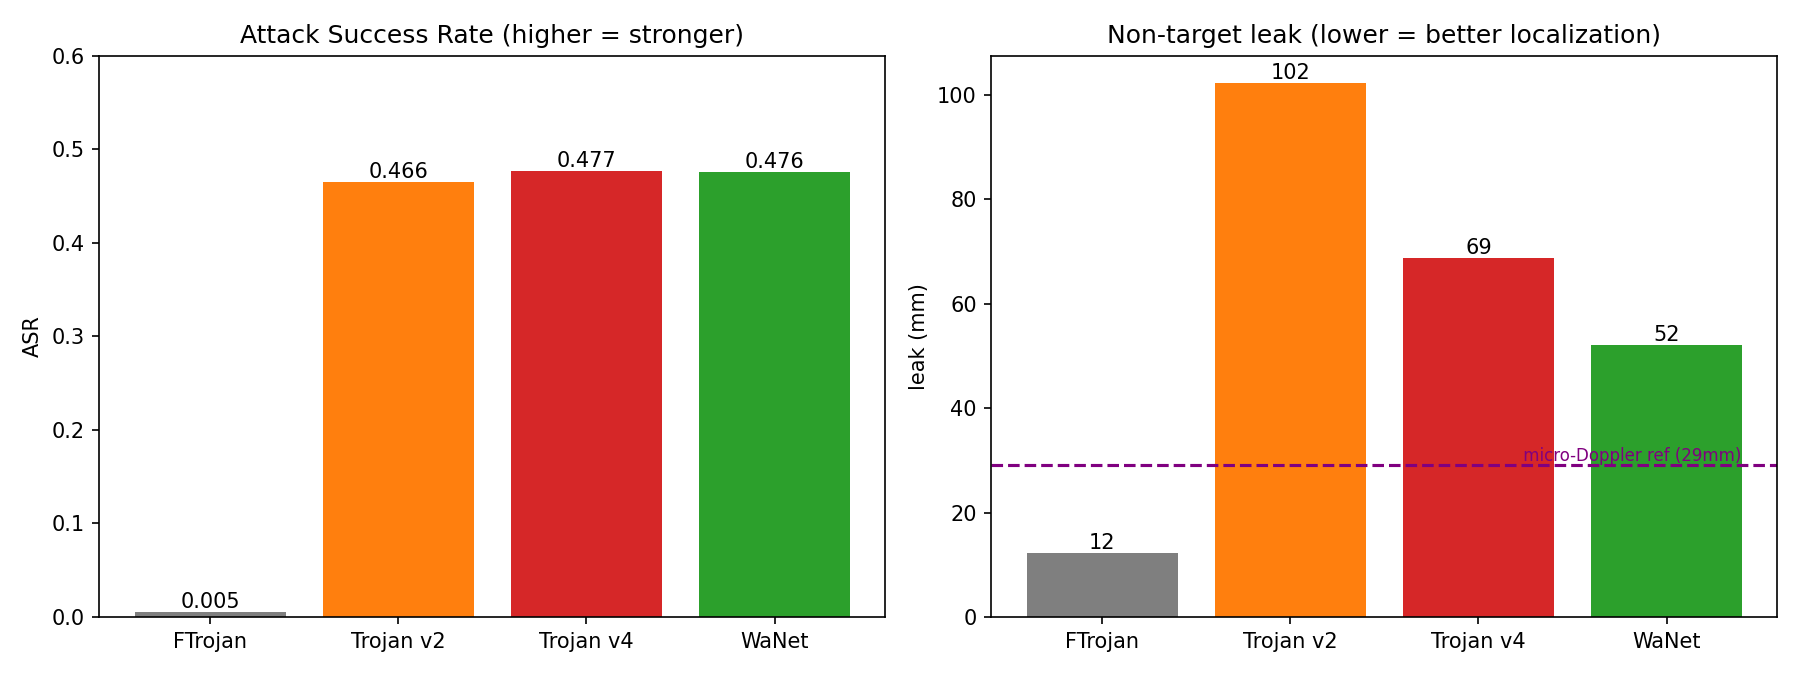
\includegraphics[width=0.9\textwidth]{fig_compare_bar.png}
\end{frame}

\begin{frame}{\textcircled{3} WaNet --- AND it is robust to defense}
  \begin{columns}
    \column{0.5\textwidth}
      \textbf{Same fine-tuning defense (30 epochs on clean data):}
      \begin{center}
      \begin{tabular}{ccc}
        \toprule
        \textbf{ep} & \textbf{Trojan} & \textbf{WaNet} \\
        \midrule
        before & 0.466 & 0.476 \\
        ep10   & \bad{0.000} & \good{0.415} \\
        ep30   & \bad{0.000} & \good{0.328} \\
        \bottomrule
      \end{tabular}
      \end{center}
      \vspace{0.5em}
      $\Rightarrow$ \bad{Trojan erased 100\%.} \good{WaNet only $-$31\% --- still alive.}
      \vspace{0.4em}

      \textbf{Why robust?} Warping distorts \emph{globally and diffusely} over the signal structure --- not localized to a few neurons like Trojan --- so fine-tuning cannot overwrite it.
    \column{0.5\textwidth}
      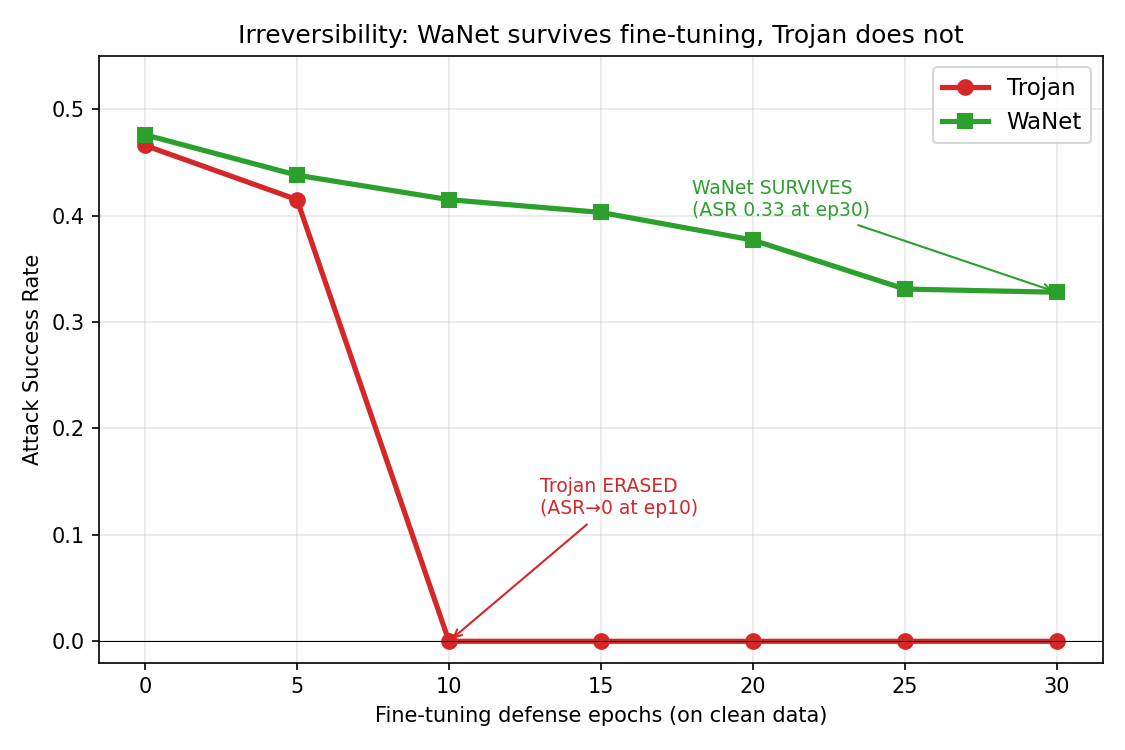
\includegraphics[width=\linewidth]{fig_defense.png}
  \end{columns}
\end{frame}

% ======================================================================
\section{Summary}
% ======================================================================

\begin{frame}{Overall comparison}
  \begin{columns}
    \column{0.54\textwidth}
      \begin{center}
      \begin{tabular}{lccc}
        \toprule
        \textbf{Method} & \textbf{ASR} & \textbf{leak} & \textbf{robust} \\
        \midrule
        FTrojan      & \bad{0.005} & 12 & --- \\
        Trojan (v4)  & 0.477 & 69 & \bad{erased} \\
        \textbf{WaNet} & \textbf{0.476} & \good{52} & \good{0.328} \\
        \bottomrule
      \end{tabular}
      \end{center}
      \vspace{0.6em}
      {\small All methods: clean PCK $\sim$0.91, Spearman = 1.0 $\to$ stealth + dose-response preserved.}
    \column{0.46\textwidth}
      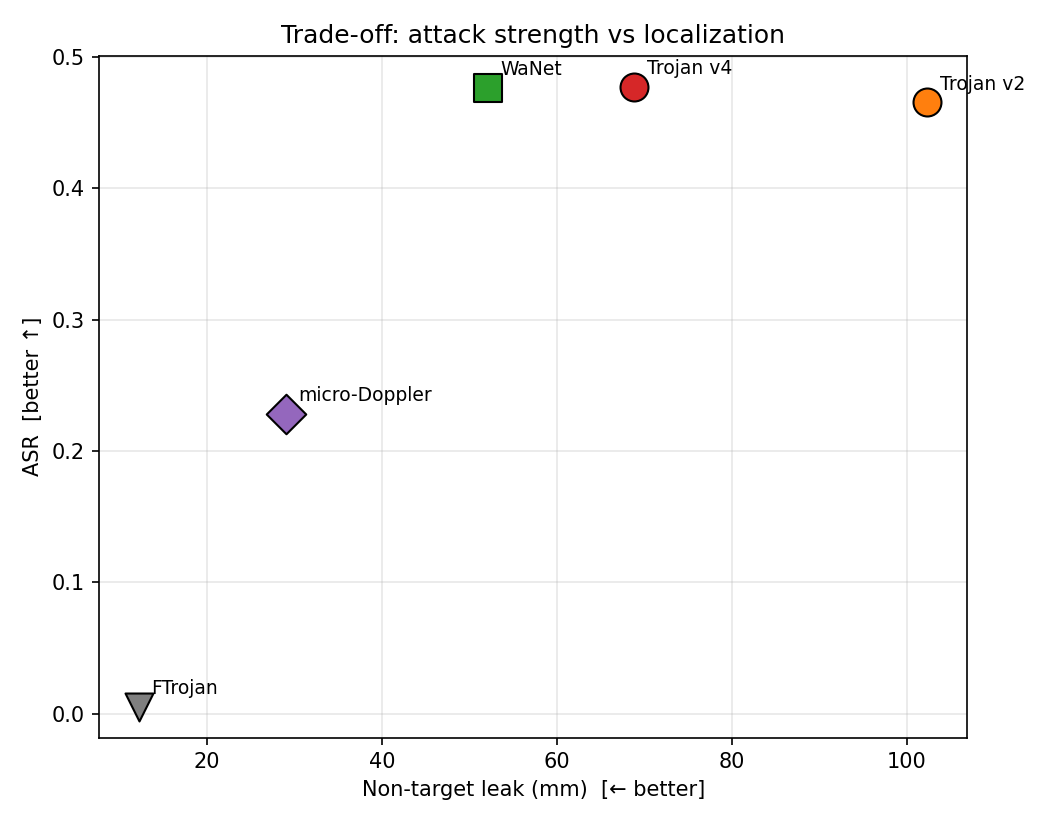
\includegraphics[width=\linewidth]{fig_tradeoff_scatter.png}
  \end{columns}
\end{frame}

\begin{frame}{Conclusion \& Contributions}
  \begin{enumerate}
    \item \acc{First} to bring an \emph{analog/dose-response} backdoor into \textbf{WiFi-CSI pose} (an unexplored gap).
    \item \textbf{Three mechanisms} adapted from vision to WiFi: frequency (FTrojan), neuron-optimized (Trojan), warping (WaNet).
    \item \textbf{Valuable negative result:} a pure frequency trigger is too weak on normalized CSI.
    \item \good{WaNet wins:} as strong as Trojan, better localized, \textbf{and robust to fine-tuning} --- Trojan is not.
    \item All methods preserve \textbf{stealth} (PCK$\sim$0.91) and \textbf{dose-response} (Spearman = 1.0).
  \end{enumerate}
  \vfill
  \begin{block}{Take-away}
    For WiFi-CSI pose, a \emph{warping} mechanism beats an \emph{optimized pattern} in both localization and robustness.
  \end{block}
\end{frame}

\begin{frame}{Appendix --- References}
  \footnotesize
  \begin{itemize}
    \item \textbf{Liu et al.}, \emph{Trojaning Attack on Neural Networks}, NDSS 2018.
    \item \textbf{Nguyen \& Tran}, \emph{WaNet --- Imperceptible Warping-based Backdoor Attack}, ICLR 2021.
    \item \textbf{Wang et al.}, \emph{An Invisible Black-box Backdoor Attack through Frequency Domain (FTrojan)}, ECCV 2022.
    \item \textbf{Liu, Dolan-Gavitt, Garg}, \emph{Fine-Pruning}, RAID 2018 (defense).
    \item \textbf{Invisibility Cloak} (2024), \textbf{6DAttack} (2024) --- camera-based pose backdoors (related).
    \item Dataset: \textbf{Person-in-WiFi-3D} (Yan et al., CVPR 2024).
  \end{itemize}
\end{frame}

\begin{frame}[plain]
  \centering
  \vfill
  {\Huge \acc{Thank you!}}\\[1em]
  {\large Q \& A}
  \vfill
\end{frame}

\end{document}
